\section{Gold-PVD}
\label{goldpvd}

Als Testsystem für PVD-Prozesse bietet sich Gold-PVD an, die zwar durch Oberflächendiffusion dominiert wird, jedoch ideale fcc-kristalline Strukturen bildet.
Die genutzte EAM-Potentialdatei stammt aus dem \todo{ref}LAMMPS-Paket, basiert aber auf Parametern von Foiles et al.\cite{foiles_embedded-atom-method_1986}, die für Einbettung einzelner Atome in Bulk- und Oberflächensysteme optimiert wurden.

\subsection{Voruntersuchungen}

Zur Validierung grundlegender Materialeigenschaften wurden Bindungslängen, Dichten und Koordinationszahlen aus einer relaxierten kristallinen Phase untersucht (Tabelle \ref{tab:goldpreresults}).
Zur Bestimmung dieser Werte wurde ein Goldkristall von \SI{40x40x40}{\angstrom} Größe auf \SI{1000}{\kelvin} aufgeheizt, im kanonischen Ensemble relaxiert und anschließend abgekühlt.
Wie man den Ergebnissen ansehen kann, bleibt die Kristallstruktur erwartungsgemäß erhalten (die Schmelztemperatur wurde für die Relaxierung nicht überschritten) und steht in guter Übereinstimmung mit Literaturwerten.
Die Parametrisierung repräsentiert somit das Zielsystem.

\begin{table}
  %% \oddrowcolors
  \caption[Eigenschaften von Gold]{Vergleich der Eigenschaften von Gold mit experimentellen und Literaturdaten als Voruntersuchung des PVD-Prozesses
    %% \todo[inline]{ref}
  }
  \label{tab:goldpreresults}
  \begin{tabularx}{\textwidth}{|lXXXX|}
    \hline
    \textbf{unters. Größe} & \textbf{Temperatur} & \textbf{Simulation} & \textbf{Experiment} & \textbf{Abweichung}\\
    \hline
    Bindungslänge  &  \SI{50}{\kelvin}   &  \SI{2.885}{\angstrom}                    &  \SI{2.884}{\angstrom}                    &  \SI{0.05}{\percent}  \\
    Koordination   &  \SI{50}{\kelvin}   &  \SI{12.00}{}                             &  \SI{12.00}{}                             &  \SI{0}{\percent}     \\
    Dichte         &  \SI{300}{\kelvin}  &  \SI{18.99}{\gram\per\cubic\centi\meter}  &  \SI{19.30}{\gram\per\cubic\centi\meter}  &  \SI{1.6}{\percent}   \\
    Dichte         &  \SI{500}{\kelvin}  &  \SI{18.89}{\gram\per\cubic\centi\meter}  &  \SI{19.13}{\gram\per\cubic\centi\meter}  &  \SI{1.2}{\percent}   \\
    \hline
  \end{tabularx}
\end{table}

%% \todo[inline]{Oberflächenvalidierung}

\subsection{Thermodynamische Eigenschaften}
\label{goldthermo}

Neben strukturellen Eigenschaften bilden EAM-Potentiale auch einige thermodynamische Eigenschaften von Metallen ab.
Für deren Untersuchung wurde die Massendichte in Abhängigkeit der Temperatur für die Teststruktur aufgenommen, die langsam auf \SI{2000}{\kelvin}, also weit über den Schmelzpunkt von \SI{1337}{\kelvin}, aufgeheizt wurde.
Die Ergebnisse (Abbildung \ref{fig:goldthermo}) zeigen gute Übereinstimmung mit experimentellen Daten, wofür Relaxationszeiten $t_\text{relax}$ oberhalb von \SI{20}{\pico\second} und Thermostat-Dämpfungsparameter $\tau$ \SI{\approx0.02}{\femto\second} als notwendig ermittelt wurden.
Bei geringeren $t_\text{relax}$ oder $\tau$ relaxiert das System innerhalb eines Temperaturschrittes nicht vollständig, wodurch der Schmelzpunkt überschätzt wird, wie in Abbildung \ref{fig:goldthermo-b} zu sehen ist.

\begin{figure}
  \captionsetup[subfigure]{singlelinecheck=false}
  \def\subfigwidth{7cm}
  \begin{subfigure}[t]{\subfigwidth}
    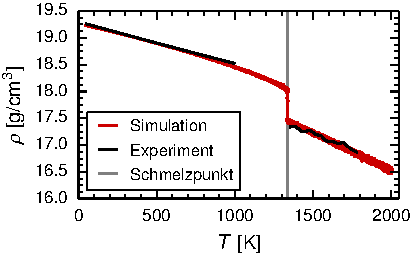
\includegraphics[width=\textwidth]{gold_bestthermo}
    \subcaption{Temperaturverlauf bei $ t_\text{relax}=\SI{50}{\pico\second}$ und $\tau=\SI{0.02}{\femto\second}$}
    \label{fig:goldthermo-a}
  \end{subfigure}
  \hfill
  \begin{subfigure}[t]{\subfigwidth}
    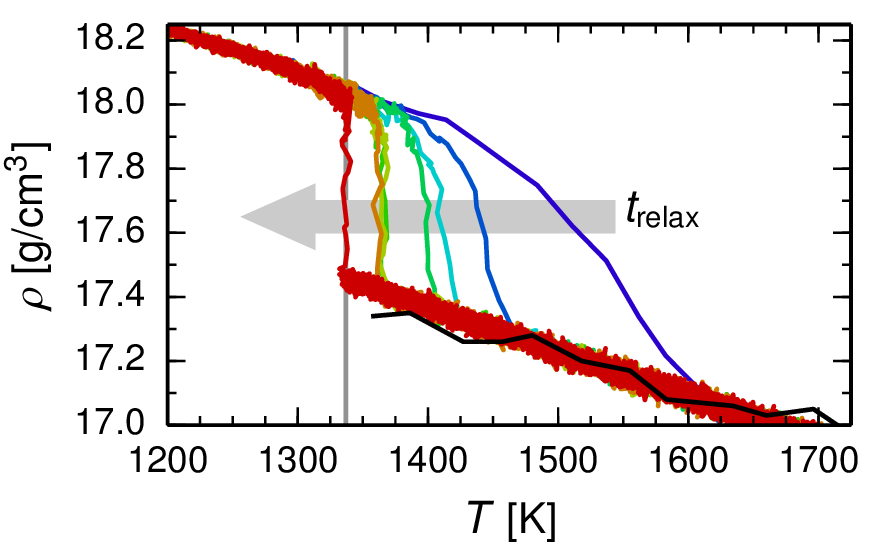
\includegraphics[width=\textwidth]{gold_relaxtime}
    \subcaption{Abhängigkeit des simulierten Schmelzpunktes von der Relaxationszeit}
    \label{fig:goldthermo-b}
  \end{subfigure}
  \caption[Ergebnisse thermodynamischer Simulationen von Gold]{Ergebnisse thermodynamischer Simulationen von Gold.
    Verlauf stimmt gut mit experimentellen Daten (schwarze Linien) überein.
    Experimentelle Werte stammen aus Standardliteratur sowie von Brillo et al.\cite{brillo_density_2006}.
  }
  \label{fig:goldthermo}
\end{figure}

\subsection{Prozess-Simulation}

Zur Simulation eines Gold-PVD-Prozesses mit Parsivald wurden die untersuchten Potentialparameter sowie ein Kristallsubstrat im PVD-Modus eingelesen und Relaxationszeiten und Größen der MD-Simulationsräume aus den Vorbetrachtungen übernommen.
Damit ergeben sich Reaktionsräume der Größe \SI{37x37x25}{\angstrom} mit jeweils ca. \num{1800} Atomen, Relaxationszeiten von \SI{1.4}{\nano\second} in \num{1400} Simulationsschritten und Auftreffgeschwindigkeiten von \SI{4}{\angstrom/\pico\second}, die aus üblichen Sputterbedingungen stammen.\todo{wie berechnet?}

Abbildung \ref{fig:golddepositions-a} zeigt, wie das Substrat unter Erhalt der Kristallstruktur fortgesetzt wird.
Poren und Einschlüsse wurden durch Untersuchung der Alphastruktur nicht gefunden.
Abbildung \ref{fig:goldroughness-a} stellt die Rauheit dar, die beim glatten Substrat über den Abscheidungszeitraum konstant geblieben ist.
Fehler- und Abbruchraten bei den LAMMPS-Berechnungen lagen mit \SI{0.25}{\percent} unterhalb des aus den ALD-Prozessen der Bachelorarbeit erwarteten Wertes von \SI{5}{\percent}

\subsubsection{Wachstum auf strukturierten Substraten}

Neben dem glatten Substrat wurden auch Abscheidungen auf strukturierten Substraten (Abbildung \ref{fig:golddepositions}) mit den gleichbleibenden Prozessbedingungen simuliert.
Als Substrate wurden Stufen oder Spitzen mit einer Höhe von jeweils \SI{20}{\angstrom} und Neigungen von \SI{15}{\degree}, \SI{20}{\degree}, \SI{30}{\degree}, \SI{45}{\degree}, \SI{60}{\degree} und \SI{90}{\degree} präpariert.
Auf vorherige Relaxierung der Substrate wurde aufgrund der Prozessstabilität sowie der relaxierenden Eigenschaften der MD-Ereignisse verzichtet.
Zusätzlich wurden Lamellen und Gitter mit einer Strukturbreite von \SI{16}{\angstrom} zur Untersuchung eventueller Prozessartefakte präpariert.

\begin{figure}
  \captionsetup[subfigure]{singlelinecheck=false}
  \def\subfigwidth{0.31\textwidth}
  \begin{subfigure}[t]{\subfigwidth}
    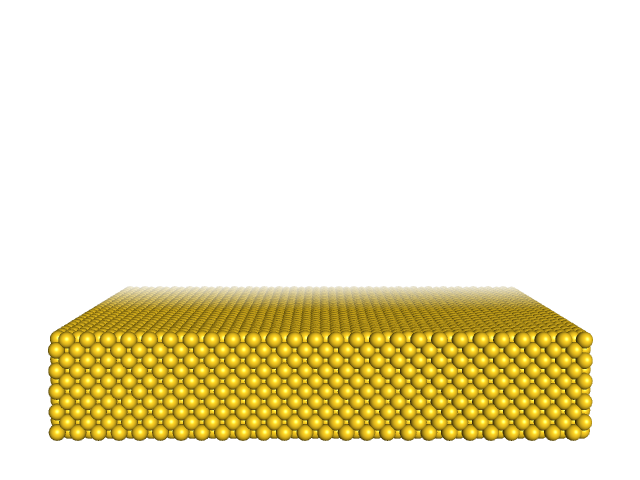
\includegraphics[width=\textwidth]{Au_substrate_flat}
    \subcaption{Glattes Gold-Substrat}
    \label{fig:golddepositions-a}
  \end{subfigure}
  \hfill
  \begin{subfigure}[t]{\subfigwidth}
    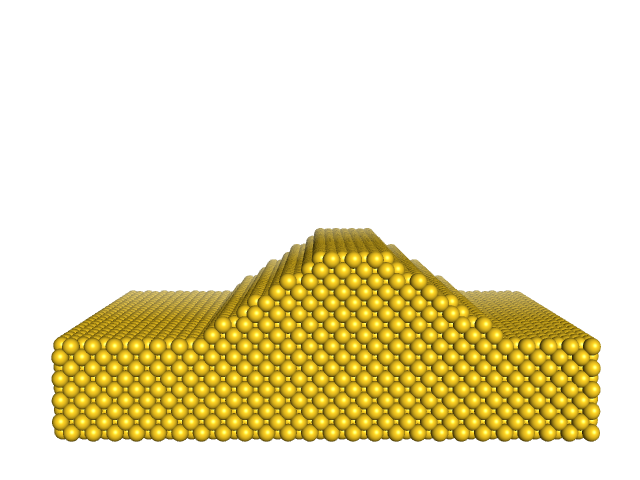
\includegraphics[width=\textwidth]{Au_substrate_step30}
    \subcaption{Gold-Stufe, \SI{30}{\degree}}
    \label{fig:golddepositions-b}
  \end{subfigure}
  \hfill
  \begin{subfigure}[t]{\subfigwidth}
    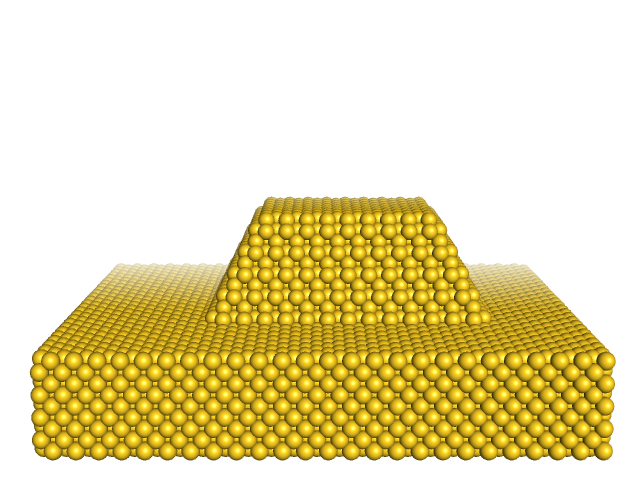
\includegraphics[width=\textwidth]{Au_substrate_tip60}
    \subcaption{Gold-Spitze, \SI{60}{\degree}}
    \label{fig:golddepositions-c}
  \end{subfigure}

  \LARGE\center{$\Downarrow$}
  \vspace{0.25cm}

  \captionsetup[subfigure]{singlelinecheck=false}
  \def\subfigwidth{0.31\textwidth}
  \begin{subfigure}[t]{\subfigwidth}
    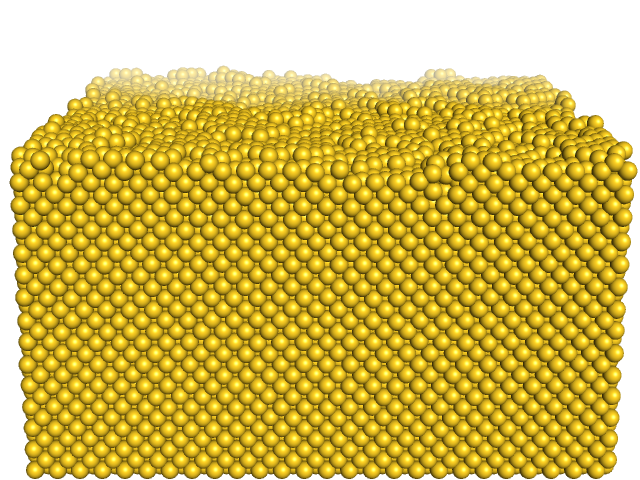
\includegraphics[width=\textwidth]{Au_deposition_flat}
    \subcaption{Glatte, kristalline Schicht ($\sigma_z = \SI{1.2}{\angstrom}$)}
    \label{fig:golddepositions-d}
  \end{subfigure}
  \hfill
  \begin{subfigure}[t]{\subfigwidth}
    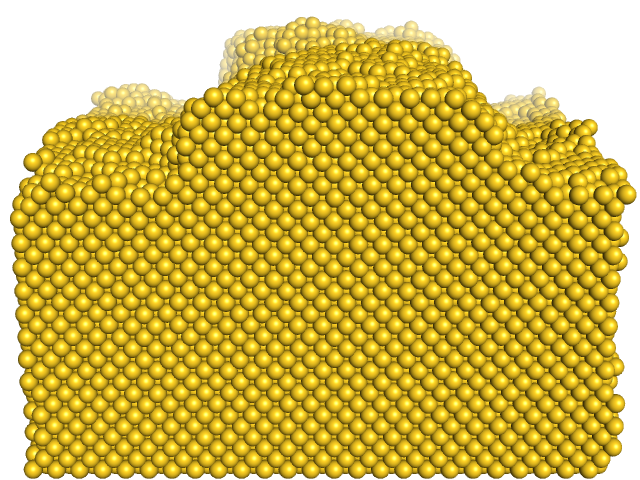
\includegraphics[width=\textwidth]{Au_deposition_step30}
    \subcaption{Fortsetzung der Stufe ($\sigma_z = \SI{6.4}{\angstrom}$)}
    \label{fig:golddepositions-e}
  \end{subfigure}
  \hfill
  \begin{subfigure}[t]{\subfigwidth}
    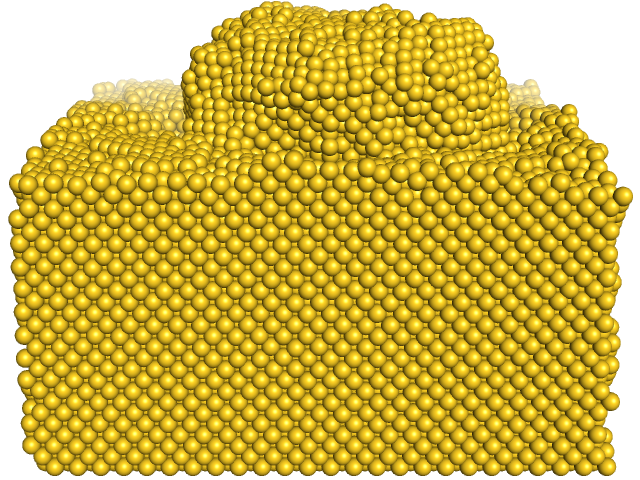
\includegraphics[width=\textwidth]{Au_deposition_tip60}
    \subcaption{Fortsetzung der Spitze ($\sigma_z = \SI{8.0}{\angstrom}$)}
    \label{fig:golddepositions-f}
  \end{subfigure}
  \caption[Gold-Abscheidung auf strukturierten Substraten]{
    Goldschicht nach 50 Abscheidungsschritten (\SI{47}{\angstrom}) auf verschiedenen Substraten
  }
  \label{fig:golddepositions}
\end{figure}

\begin{figure}
  \captionsetup[subfigure]{singlelinecheck=false}
  \def\subfigwidth{0.49\textwidth}

  \begin{subfigure}[t]{\subfigwidth}
    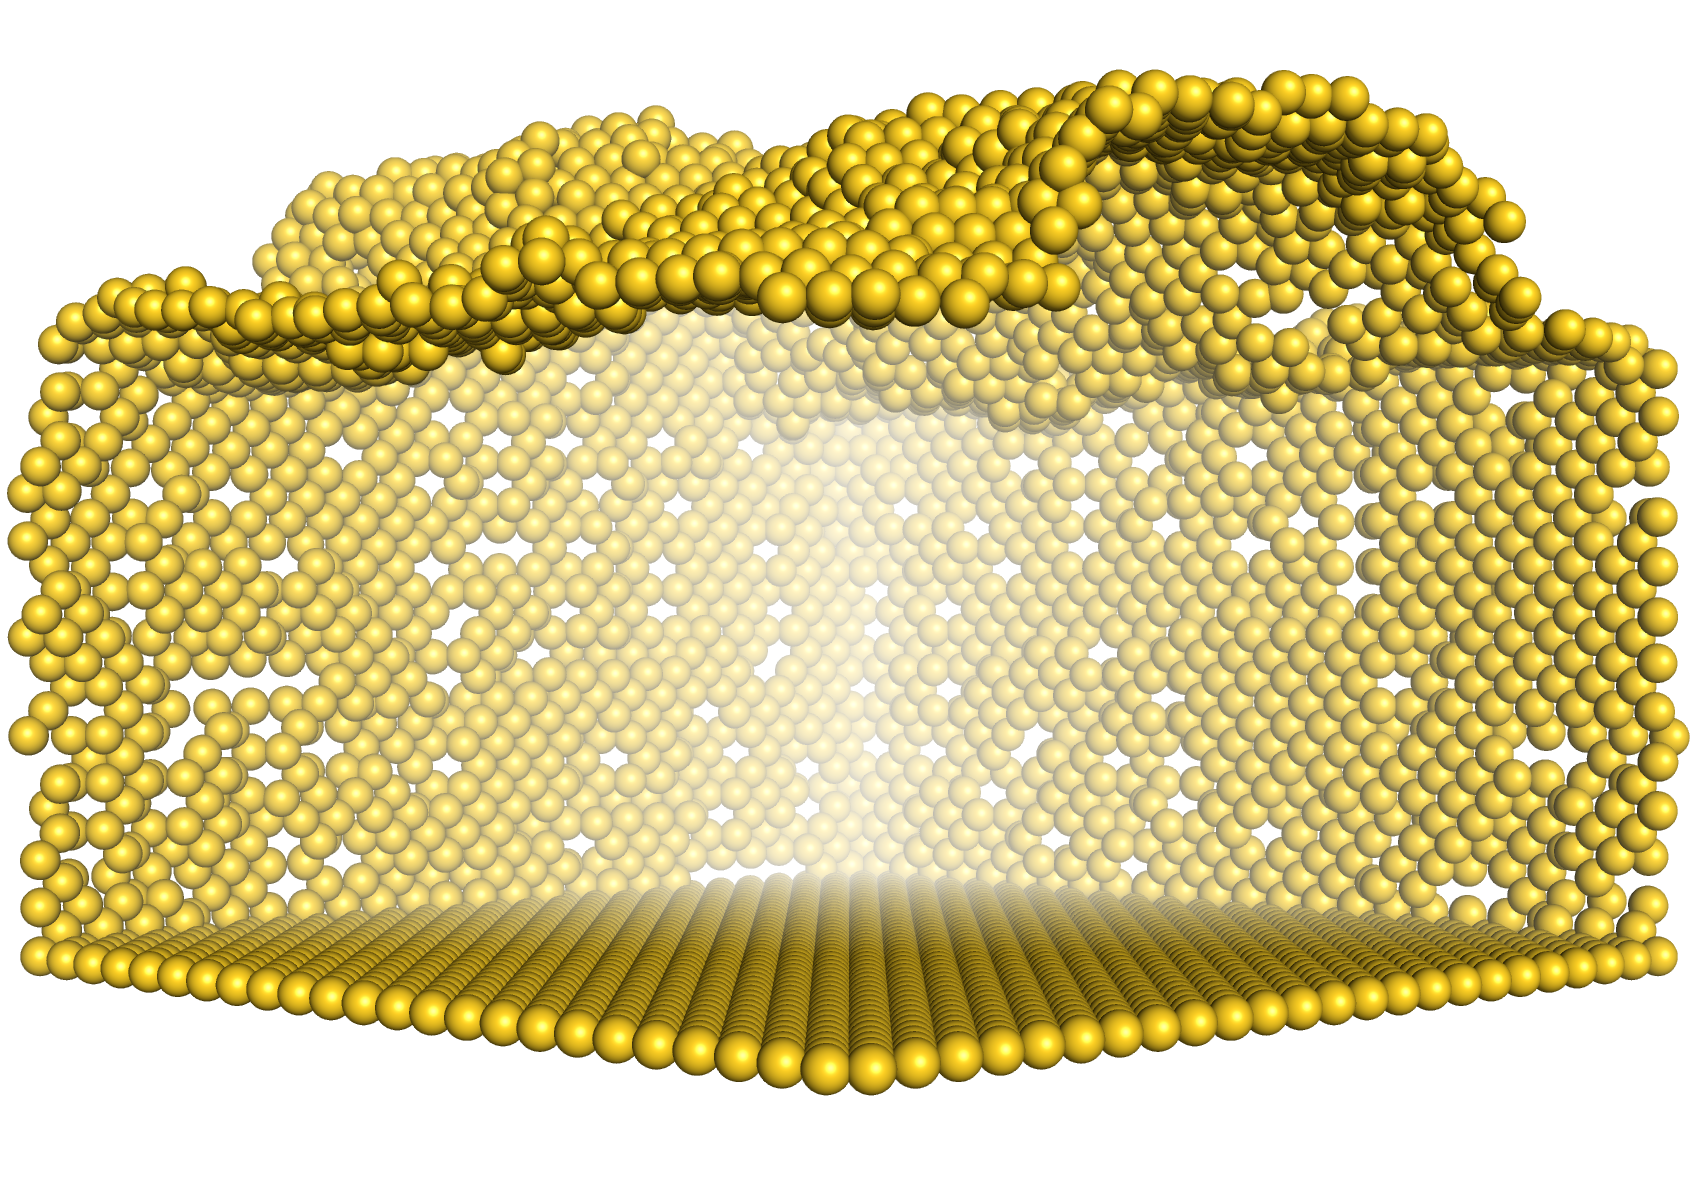
\includegraphics[width=\textwidth]{gold_step30_pockets}
    \subcaption{\SI{30}{\degree}-Stufe: Keine Poren oder Einschlüsse}
    \label{fig:goldpockets-a}
  \end{subfigure}
  \hfill
  \begin{subfigure}[t]{\subfigwidth}
    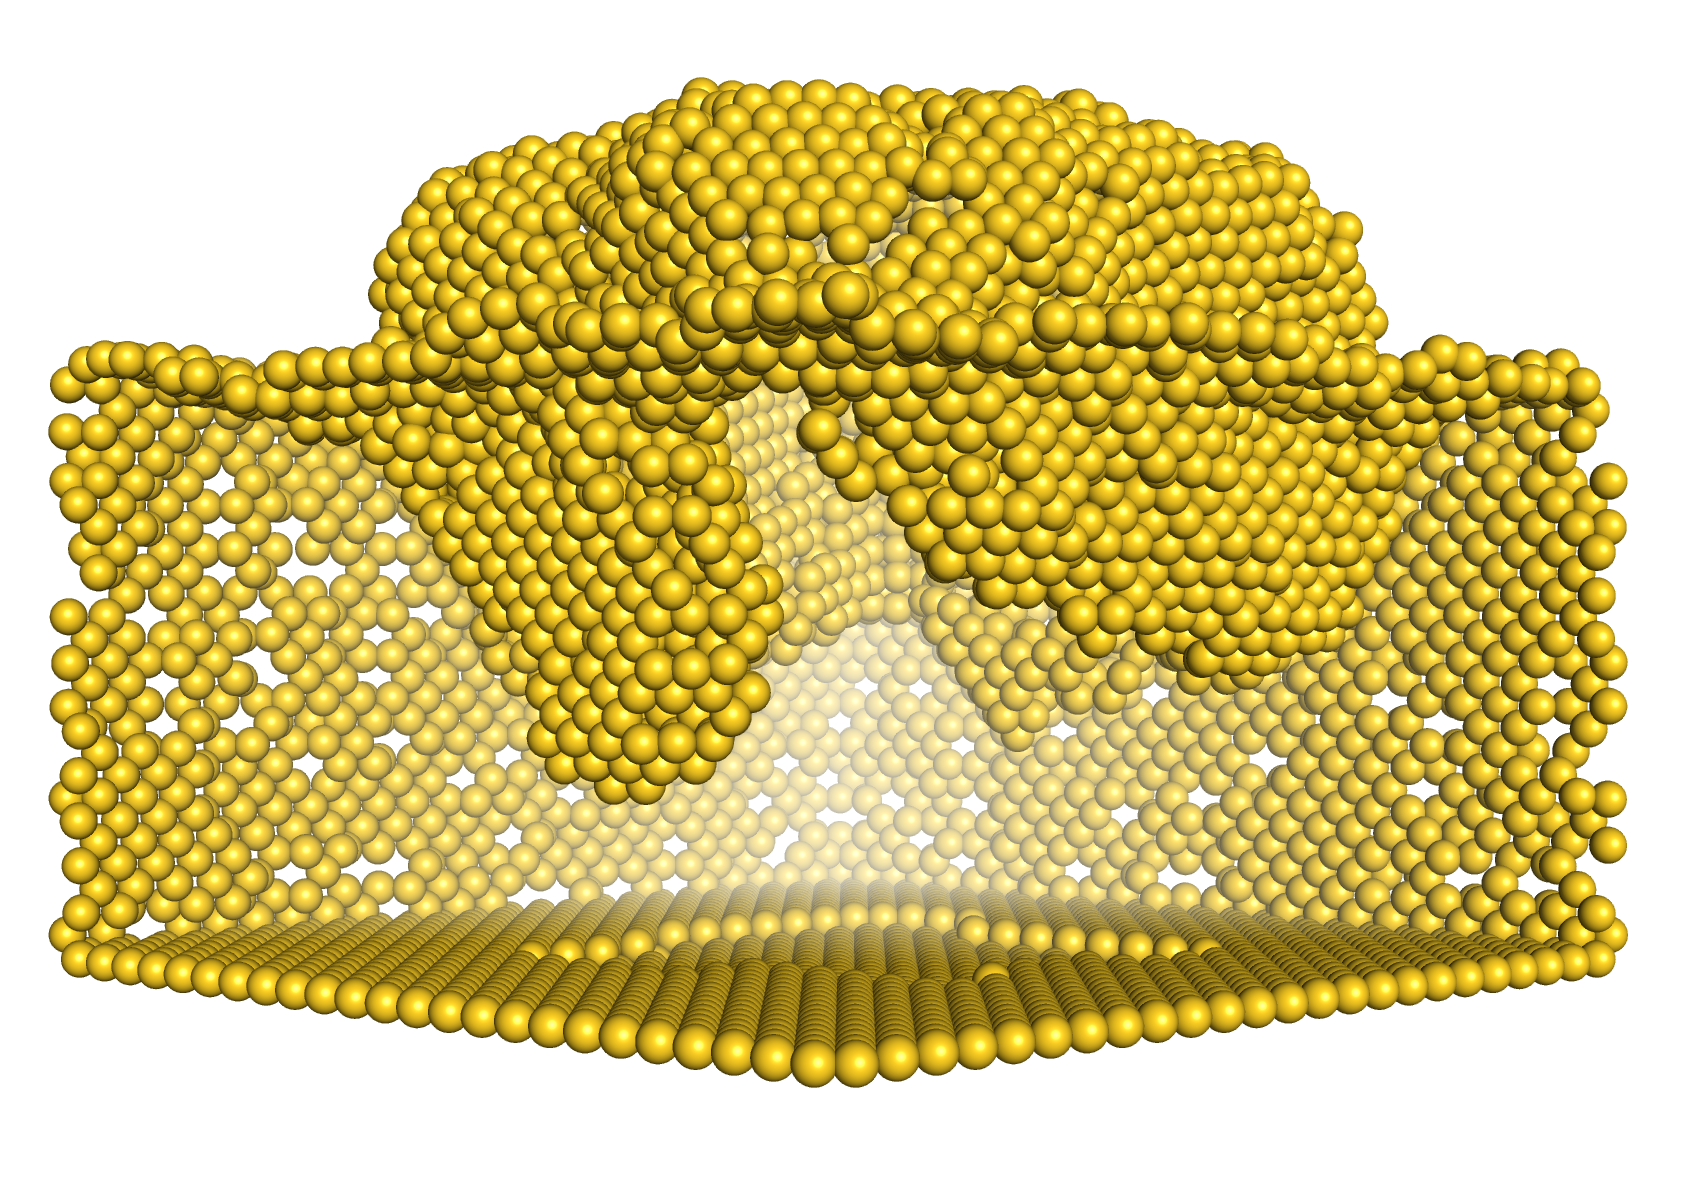
\includegraphics[width=\textwidth]{gold_tip90_pockets}
    \subcaption{Porenbildung an der Basis der \SI{90}{\degree}-Spitze}
    \label{fig:goldpockets-b}
  \end{subfigure}

  \caption[Porenbildung bei Gold-Strukturen]{Porenbildung bei Gold-Strukturen nach 40 Abscheidungsschritten (ca. \num{22000} PVD-Ereignisse $\hat{=}$ \SI{38}{\angstrom}).
  }
  \label{fig:goldpockets}
\end{figure}

Wie man den Alpha-Formen der simulierten Strukturen (Abbildung \ref{fig:goldpockets-a}) entnehmen kann, beinhaltet das abgeschiedene Gold bei geringen Neigungswinkeln keine Kristalldefekte, Poren oder Einschlüsse.
Bei Abscheidungen auf Substrate hoher Neigungswinkel (>\SI{60}{\degree}) bilden sich Poren mit größerer Ausdehnung (>\SI{20}{\angstrom}).
Durch Bildung von Überhängen an den Stufen werden die Poren zu Hohlräumen abgeschlossen, die nicht durch Relaxierung geschlossen werden.
Dies zeigt sich auch in den Oberflächenrauheiten der untersuchten Strukturen (Abbildung \ref{fig:goldroughness}).

\subsection{Vergleich mit gesputterten Schichten}

AFM-Untersuchungen gesputterter Goldschichten zeigen polykristallines Wachstum mit Rauheiten im Bereich von \SI{1.1}{\nano\meter} (etwa drei fcc-Kristallschichten)\cite{svorcik_annealing_2011}.
Dabei wird die Oberflächenrauheit von der Bildung von Nanopartikeln dominiert, deren Schmelztemperaturen mit der Größe der Partikel zunehmen\cite{liu_melting_2001}.
Kleinere Goldpartikeln verschmelzen oberhalb ihrer spezifischen Schmelztemperatur zu größeren Partikeln, wodurch die Rauheit der Goldoberfläche mit höheren Substrat- oder Annealing-Temperaturen zunimmt.
Bei \todo{Vergleich womit?}vergleichsweise niedrigen Temperaturen, wie sie bei Sputtering vorhanden sind, werden durch Unterbindung der Verschmelzung kleiner Goldpartikel geringere Rauheiten erreicht, die mit längerer Sputterdauer weiter abnehmen\cite{svorcik_annealing_2011}.

In Parsivald-Simulationen ist dieser Trend bisher nur selten zu beobachten, wie etwa bei der \SI{45}{\degree}-Spitze, deren Rauheit gegen Ende der Simulation langsam abnimmt.
Die Systeme wachsen in monokristallinen Schichten entlang der Kristallebenen, jedoch zeigen Abscheidungssimulationen auf einigen strukturierten Substraten zusätzliche Porenbildung an Überhängen, die in der aktuellen Oberflächensuche begründet sind.
So wird die Oberfläche und damit mögliche Ereignisorte parallel zur Z-Achse gesucht, anstatt die Alpha-Form über eine Delaunay-Triangulation der Atompositionen zu ermitteln, wie es zur bereits Auswertung der simulierten Strukturen durchgeführt wird.
Somit werden höher gelegene Ereignisorte in der direkten Nachbarschaft bevorzugt, was sich in der Verstärkung von Überhängen bei strukturierten Substraten mit hohen Neigungswinkeln zeigt (Abbildung \ref{fig:goldpockets-b}).
Als Lösung bieten sich die eben genannten Alpha-Formen an, welche jedoch erst für das Parsivald-Modell optimiert werden müssen (Abschnitt \ref{datadelaunay}).

Bei der Analyse der simulierten Strukturen wurde bei Abscheidungen auf glatten Substraten eine Rauheit von \SI{0.12}{\nano\meter} ermittelt, welche nur ca. \SI{10}{\percent} der experimentellen Werte beziehungsweise einer Lage von Goldatomen entspricht.
Strukturierte Substrate zeigen hier höhere Rauheiten, die zwar den experimentell bestimmten Rauheiten entsprechen (Abbildung \ref{fig:goldroughness}), aber ebenfalls keine Nanopartikel enthalten, sondern aus monokristallinen Schichten bestehen.
Daran lässt sich erkennen, dass die verwendeten \todo{word}MD-Simulation-Boxen zu klein und die Relaxationszeiten zu kurz sind, um die Bildung von Nanopartikeln darstellen zu können.
Zusätzlich verhindern kleine MD-Boxen in Verbindung mit monokristallinen Substraten die Ausbildung polykristalliner Strukturen, was sich im Wachstum monokristalliner Schichten äußert.
Derartige Finite-Size-Effekte sind Molekulardynamik-Simulationen inhärent, werden jedoch durch Parsivald für einige Systeme zusätzlich verstärkt.
Bei Abscheidung amorpher Schichten, wie für CVD- und ALD-Prozesse üblich, konnte dieser Effekt bisher nicht beobachtet werden (Abschnitt \ref{siliconpvd}).

\begin{figure}
  \captionsetup[subfigure]{singlelinecheck=false}
  \def\subfigwidth{0.49\textwidth}

  \begin{subfigure}[t]{\subfigwidth}
    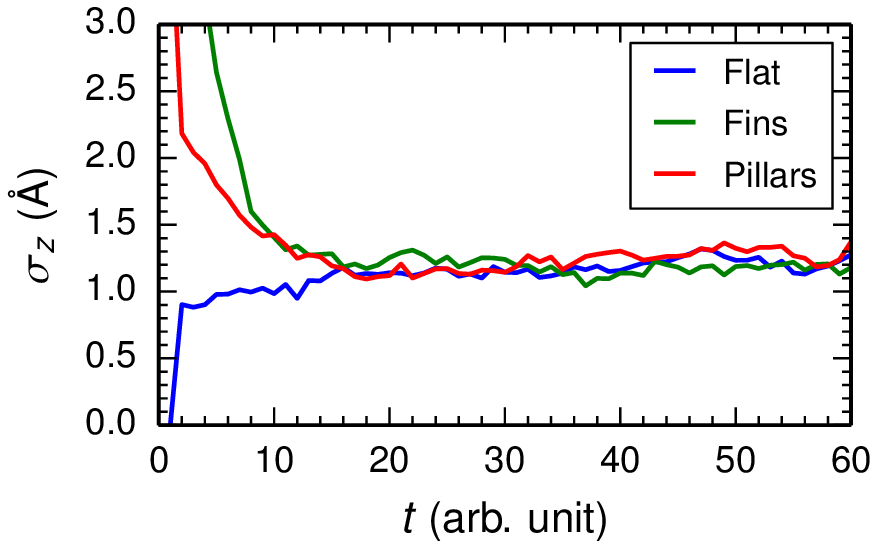
\includegraphics[width=\textwidth]{gold_goodroughness}
    \subcaption{Zeitverlauf der Rauheit von glatten (Flat) und fein strukturierten Oberflächen (Fins, Pillars: \SI{10}{\angstrom} breite Erhebungen)}
    \label{fig:goldroughness-a}
  \end{subfigure}
  \hfill
  \begin{subfigure}[t]{\subfigwidth}
    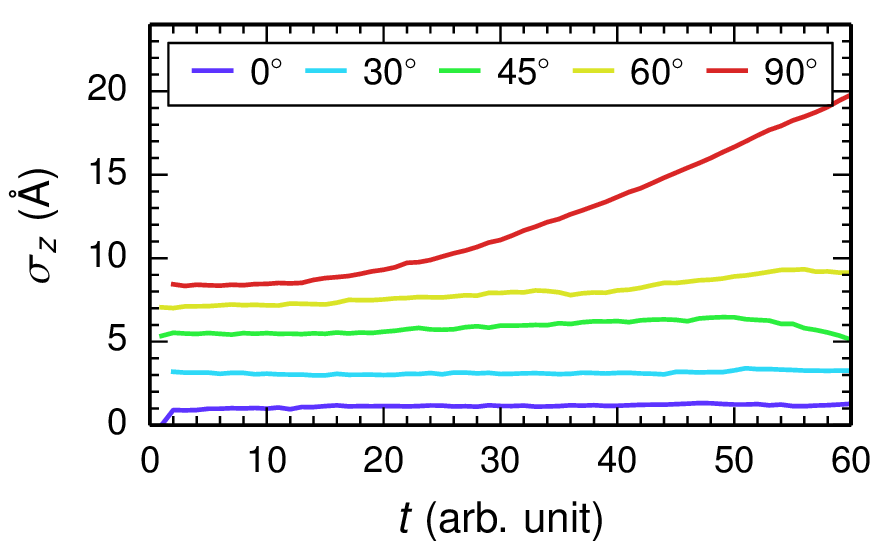
\includegraphics[width=\textwidth]{gold_tiproughness}
    \subcaption{Zeitverlauf der Rauheit von \SI{50}{\angstrom} breiten Spitzen variabler Steigung.
      Oberflächenrauheiten werden nicht verringert
    }
    \label{fig:goldroughness-b}
  \end{subfigure}

  \caption[Oberflächenrauheit von Gold]{Oberflächenrauheit von Gold.
    Im idealen Fall konvergiert die Rauheit gegen einen konstanten Wert von \SI{1.2}{\angstrom}
  }
  \label{fig:goldroughness}

\end{figure}

\subsection{Skalierbarkeit mit der Simulationsgröße}

Die Größe der simulierten Strukturen, wie sie beispielsweise für Beschichtungen kompletter \todo{Nanodevice}Nano-Bauelemente von Interesse sind, ist bei jeder Simulationsmethode durch verschiedene Einflüsse wie Speicherbedarf und Laufzeit limitiert.
Allgemein lässt sich sagen, dass präzisere Methoden nur auf kleineren Systemen und kürzeren Zeitskalen funktionieren (Abbildung \ref{fig:methodscales}).
Atomistische Methoden, insbesondere die Molekulardynamik, sind von theoretischer Seite durch die Notwendigkeit der paarweisen Interaktionen und von technischer Seite durch Speicher- und Netzwerkbandbreite begrenzt.
Somit sind Systeme mit mehr als \num{100000} Atomen nur mit hohem Aufwand über viele Zeitschritte hinweg berechenbar.
Die in Abschnitt \ref{datastructures} vorgestellten Überlegungen zur Optimierung, in Kombination mit dem Parallelisierungsansatz des Parsivald-Modelles aus Abschnitt \ref{parsivald}, sollen hier einem praktischen Test unterzogen werden.

Dazu werden verschiedene quadratische Substrate mit Breiten von \SI{100}{\angstrom}, \SI{200}{\angstrom}, \SI{500}{\angstrom}, \SI{1000}{\angstrom} und \SI{10000}{\angstrom} und \SI{20000}{\angstrom} auf Speicherbedarf, Laufzeit, Anzahl der Atome und Ereignisse, Zahl gleichzeitig aktiver Worker und Bedeckungsgrad der Oberfläche mit aktiven Ereignissen untersucht (Tabelle \ref{tab:goldscalability}).

\begin{table}\begin{threeparttable}

    \caption[asd]{Untersuchungen zur Skalierbarkeit des Systemes}
    \label{tab:goldscalability}

    \begin{tabularx}{\textwidth}{|Xrrrrrrr|}
      \hline
      \textbf{Größe}\tnote{2}  &  \textbf{Wachst.}     &  \textbf{Atome}  &  \textbf{Ereignisse}  &  \textbf{Worker}\tnote{a}  ~            &  \textbf{Bed.}\tnote{e}  &  \textbf{Laufzeit}  &  \textbf{RAM}\tnote{f}  \\
      \hline
      \SI{106}{\angstrom}      &  \SI{70}{\angstrom}   &  \num{59549}     &  \num{46030}          &  \num{1.8}\tnote{b}        (\num{4})    &  \SI{21.9}{\percent}     &  \SI{32.2}{\hour}   &  \SI{254}{\mebi\byte}   \\
      \SI{204}{\angstrom}      &  \SI{42}{\angstrom}   &  \num{152374}    &  \num{102374}         &  \num{14.5}\tnote{b}       (\num{18})   &  \SI{47.7}{\percent}     &  \SI{25.5}{\hour}   &  ~                      \\
      \SI{204}{\angstrom}      &  \SI{42}{\angstrom}   &  \num{152374}    &  \num{102374}         &  \num{14.5}\tnote{b}       (\num{18})   &  \SI{47.7}{\percent}     &  \SI{25.5}{\hour}   &  \SI{257}{\mebi\byte}   \\
      \SI{500}{\angstrom}      &  \SI{93}{\angstrom}   &  \num{1708600}   &  \num{1401081}        &  \num{24.8}                (\num{50})   &  \SI{13.6}{\percent}     &  \SI{73.6}{\hour}   &  \SI{282}{\mebi\byte}   \\
      \SI{1000}{\angstrom}     &  \SI{5.4}{\angstrom}  &  \num{1591908}   &  \num{381588}         &  \num{44.8}                (\num{46})   &  \SI{6.1}{\percent}      &  \SI{1.5}{\hour}    &  \SI{368}{\mebi\byte}   \\
      \SI{1000}{\angstrom}     &  ~                    &  \num{6733948}   &  \num{5539942}        &  \num{75.4}                (\num{149})  &  \SI{10.3}{\percent}     &  \SI{97.5}{\hour}   &  ~                      \\
      \SI{1}{\micro\meter}     &  \SI{1.3}{\angstrom}  &  \num{1.3e8}     &  \num{8186990}        &  \num{25.4}\tnote{c}       (\num{46})   &  \SI{0.03}{\percent}     &  \SI{117.5}{\hour}  &  \SI{11.5}{\gibi\byte}  \\
      \SI{2}{\micro\meter}     &  \SI{0.4}{\angstrom}  &  \num{4.9e8}     &  \num{10356031}       &  \num{26.3}\tnote{c}       (\num{46})   &  \SI{0.009}{\percent}    &  \SI{117.5}{\hour}  &  ~                      \\
      \SI{2}{\micro\meter}     &  \SI{1.0}{\angstrom}  &  \num{5.1e8}     &  \num{25855695}       &  \num{189}\tnote{d}        (\num{245})  &  \SI{0.06}{\percent}     &  \SI{186.8}{\hour}  &  \SI{45.4}{\gibi\byte}  \\
      \SI{4}{\micro\meter}     &  ~                    &  \num{1.9e9}     &  ~                    &  ~                         ~            &  ~                       &  ~                  &  \SI{182}{\gibi\byte}   \\
      \hline
    \end{tabularx}

    \begin{tablenotes}
    \item[2] Breite der quadratischen Oberfläche
    \item[a] Mittelwert und Maximum der zeitgleich bearbeiteten Ereignisse
    \item[b] Maximale Ereignisdichte erreicht.
      Restliche Worker sind im Wartezustand.
    \item[c] Inzwischen behobener Fehler im Host-Code hat Workerneustart verhindert
    \item[d] Maximale Bandbreite des Hosts erreicht.
      Längere MD-Simulationen erlauben mehr Worker.
    \item[e] Bedeckung: Anteil der von laufenden Ereignissen abgedeckten Oberfläche
    \item[f] Vom Hostprozess verbrauchten
    \end{tablenotes}

\end{threeparttable}\end{table}

Mit \SI{94}{\byte} pro Atom, zusätzlich zum konstanten Programmspeicher von \SI{253}{\mebi\byte}, können auch extreme Simulationsräume mit 2 Milliarden Atomen auf einer Oberfläche von \SI{4x4}{\micro\meter} vom Arbeitsspeicher moderner Hochleistungsrechner verwaltet werden können.

Anders sieht es bei der notwendigen Rechenleistung aus:
Während kleine Simulationsräume (\SI{<200}{\angstrom}) nicht wesentlich von der parallelen Rechenleistung profitieren können, scheitern größere Prozesse am Mangel daran:
Im zweiten Test mit einer \SI{2x2}{\micro\meter} großen Struktur wurde die Grenze der Bandbreite des Hostprozesses erreicht:
Die Tests haben gezeigt, dass dieser \num{38.4} Ereignisse pro Sekunde vorbereiten, starten und auswerten kann.
Mit \SI{4.86}{\second} Laufzeit pro Gold-PVD-Ereignis kann der Hostprozess aber nur 189 parallele Worker dauerhaft mit Ereignissen versorgen.
Die eigentliche Beschränkung liegt folglich in der genutzten Potentialart:
Kompliziertere und damit langsamere Potentiale, wie die später genutzten ReaxFF-Potentiale, benötigen meist mehr als \SI{30}{\second} für ein Ereignis, in extremen Fällen sogar \SI{5}{\minute}.
Somit erlauben sie theoretisch \num{1152} beziehungsweise \num{11520} parallele Worker und übersteigen damit die Möglichkeit dessen, was einem einzelnen Nutzer an einem Hochleistungsrechencluster zur Verfügung steht.
Leider erhöht sich damit auch die insgesamt benötigte Rechenzeit linear.

Die verbleibende Einschränkung wird somit von den verfügbaren Rechenkernen gebildet.
In Simulationen mit Substratgrößen auf der Mikrometer-Skala wurden nur kleine Teile der Oberfläche (\SI{<0.1}{\percent}) zeitgleich von Ereignissen simuliert.
Bei Oberflächen von \SI{2x2}{\micro\meter} Größe sind in dichtester Packung der MD-Boxen mit je \SI{37x37}{\angstrom} Größe maximal \num{291600} parallele Ereignisse möglich.
Tatsächlich werden aufgrund der Überdeckung der Ereignisse durch die zufällige Wahl der Reaktionsorte häufig \SI{<40}{\percent} davon zeitgleich simuliert.
Dennoch liegt die Zahl der verfügbaren Prozessorkerne um Größenordnungen unterhalb des optimalen Wertes, was sich in langen Simulationslaufzeiten äußert (\SI{186.8}{\hour} für \SI{1.0}{\angstrom}).

Zusammenfassend lässt sich sagen, dass Systeme mit einer Größe zwischen \SI{50x50}{\nano\meter} und \SI{300x300}{\nano\meter} mit modernen Computerclustern effizient berechenbar sind, wo hingegen kleinere Systeme nicht signifikant von der Effizienzsteigerung profitieren können und für größere Systeme die notwendige Rechenleistung unerreichbar bleibt.

